%%%%%%%%%%%%%%%%%%%%%%%%%%%%%%%%%%%%%%%%%
% University/School Laboratory Report
% LaTeX Template
% Version 3.1 (25/3/14)
%
% This template has been downloaded from:
% http://www.LaTeXTemplates.com
%
% Original author:
% Linux and Unix Users Group at Virginia Tech Wiki 
% (https://vtluug.org/wiki/Example_LaTeX_chem_lab_report)
%
% License:
% CC BY-NC-SA 3.0 (http://creativecommons.org/licenses/by-nc-sa/3.0/)
%
%%%%%%%%%%%%%%%%%%%%%%%%%%%%%%%%%%%%%%%%%

%----------------------------------------------------------------------------------------
%	PACKAGES AND DOCUMENT CONFIGURATIONS
%----------------------------------------------------------------------------------------

\documentclass{article}

\usepackage[version=3]{mhchem} % Package for chemical equation typesetting
\usepackage{siunitx} % Provides the \SI{}{} and \si{} command for typesetting SI units
\usepackage{graphicx} % Required for the inclusion of images
\usepackage{natbib} % Required to change bibliography style to APA
\usepackage{amsmath} % Required for some math elements 
\usepackage[left=3cm,top=3cm,right=3cm,bottom=3cm]{geometry} %%Márgenes
\usepackage[section]{placeins}
% Paquetes a usar
%\usepackage[spanish]{babel}   %%para Colocar el Español
\usepackage[utf8]{inputenc} %%para usar tildes adecuadamente
\usepackage{amssymb}          % Símbolos
\usepackage{hyperref}         % Vinculos 
\usepackage{graphics}         % Subfiguras
\usepackage{pdfpages}         % incluir PDF
\usepackage[tight,footnotesize]{subfigure}
\usepackage[spanish]{babel}   %%para Colocar el Español
\usepackage{pgfplots}

\renewcommand{\contentsname}{Tabla de contenido}
\renewcommand{\partname}{Parte}
\renewcommand{\appendixname}{Apéndice}
\renewcommand{\bibname}{Referencias}
\renewcommand{\figurename}{Figura}
\renewcommand{\listfigurename}{Índice de figuras}
\renewcommand{\tablename}{Tabla}
\renewcommand{\listtablename}{Índice de tablas}

\let\cleardoublepage\clearpage %Quitar paginas en blanco
\setlength{\parindent}{0pt} % Quitar sangria del inici de parrafo


\setlength\parindent{0pt} % Removes all indentation from paragraphs

\renewcommand{\labelenumi}{\alph{enumi}.} % Make numbering in the enumerate environment by letter rather than number (e.g. section 6)

%\usepackage{times} % Uncomment to use the Times New Roman font

%----------------------------------------------------------------------------------------
%	DOCUMENT INFORMATION
%----------------------------------------------------------------------------------------

\title{Imágenes y Visión - Taller 4: Taller práctico de procesamiento de imágenes} % Title

\author{
  José Francisco Molano Pulido\\
  \texttt{jf.molano1587@uniandes.edu.co}
  \and
  Sergio Daniel Hernández Charpak\\
  \texttt{sd.hernandez204@uniandes.edu.co}
}

\date{\today} % Date for the report

\pgfplotsset{compat=1.13} 
\begin{document}

\maketitle % Insert the title, author and date

\tableofcontents
% If you wish to include an abstract, uncomment the lines below
% \begin{abstract}
% Abstract text
% \end{abstract}

\newpage
%----------------------------------------------------------------------------------------
%	Filtros lineales de detección de contornos - Sergio
%----------------------------------------------------------------------------------------

\section{Filtros lineales de detección de contornos}

Primero observamos los resultados al aplicar el Operador de Sobel en la dirección Y.

\begin{figure}[ht]
\begin{center}
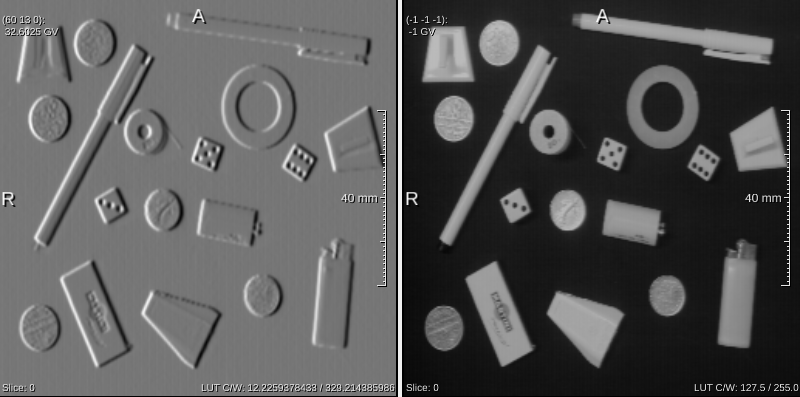
\includegraphics[width=0.7\textwidth]{1Filtros/1_sobel_y_orig.png} % Include the image placeholder.png
\caption{Imagen original y su gradiente tipo Sobel en la dirección y}
\label{fg:sobel_y}
\end{center}
\end{figure}
\FloatBarrier

Podemos observar que las fronteras sobresaltan y que son más claras para las fronteras verticales. Como los límites de los objetos no son perfectamente verticales (u horizontales) se obtienen los contornos completos de los objetos.\\
Los resultados al aplicar el Operador de Sobel en la dirección X son equivalentes, pero clarificando las fronteras horizontales.

\begin{figure}[ht]
\begin{center}
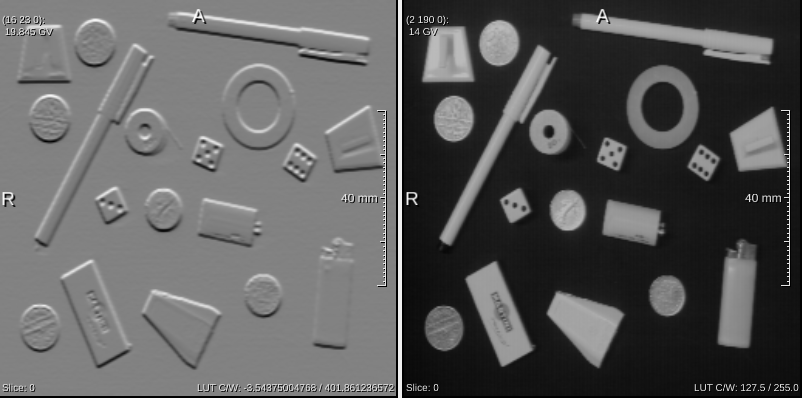
\includegraphics[width=0.7\textwidth]{1Filtros/1_sobel_x_orig.png} % Include the image placeholder.png
\caption{Imagen original y su gradiente tipo Sobel en la dirección x}
\label{fg:sobel_x}
\end{center}
\end{figure}
\FloatBarrier

Finalmente podemos observar el resultado final.

\begin{figure}[ht]
\begin{center}
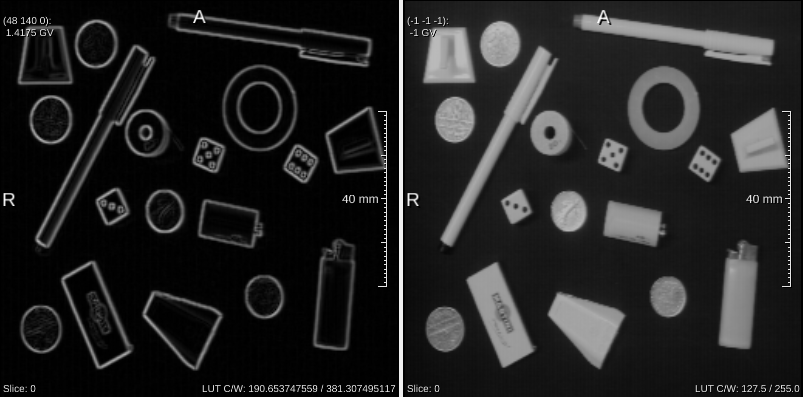
\includegraphics[width=0.7\textwidth]{1Filtros/1_sobel_grad.png} % Include the image placeholder.png
\caption{Imagen original y su gradiente tipo Sobel}
\label{fg:sobel_grad}
\end{center}
\end{figure}
\FloatBarrier

Ahora observemos los resultados al aplicar el Operador de Prewitt en la dirección Y.

\begin{figure}[ht]
\begin{center}
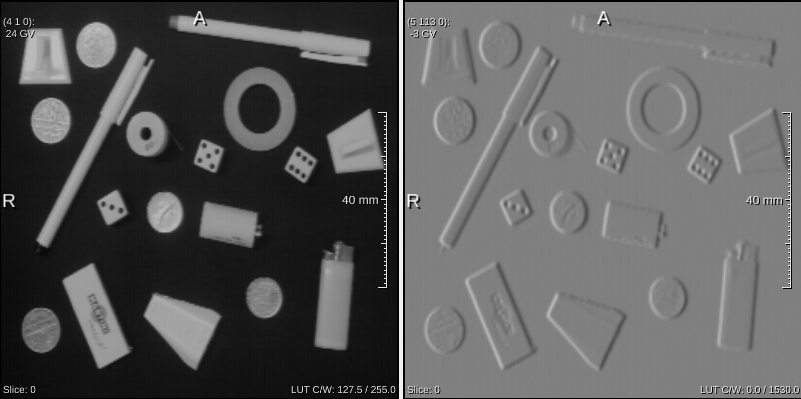
\includegraphics[width=0.7\textwidth]{1Filtros/1_prew_y.png} % Include the image placeholder.png
\caption{Imagen original y su gradiente tipo Prewitt en la dirección y}
\label{fg:prew_y}
\end{center}
\end{figure}
\FloatBarrier
Podemos observar que son resultados similares que con el operador Sobel. Lo mismo podemos
decir del operador Prewitt en la dirección x.

\begin{figure}[ht]
\begin{center}
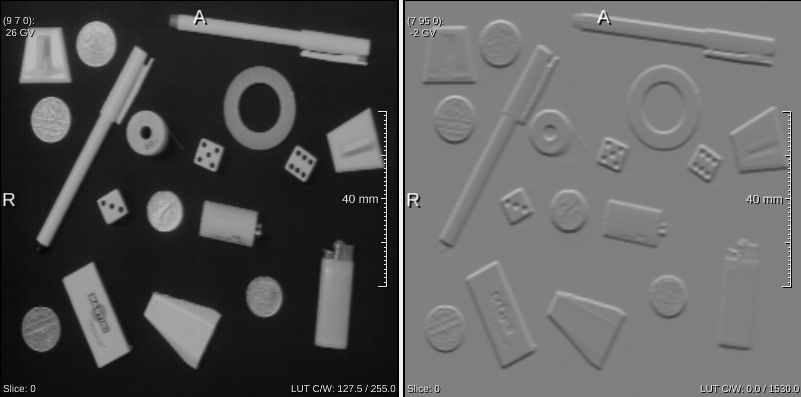
\includegraphics[width=0.7\textwidth]{1Filtros/1_prew_x.png} % Include the image placeholder.png
\caption{Imagen original y su gradiente tipo Prewitt en la dirección x}
\label{fg:prew_x}
\end{center}
\end{figure}
\FloatBarrier

Y finalmente de su gradiente:

\begin{figure}[ht]
\begin{center}
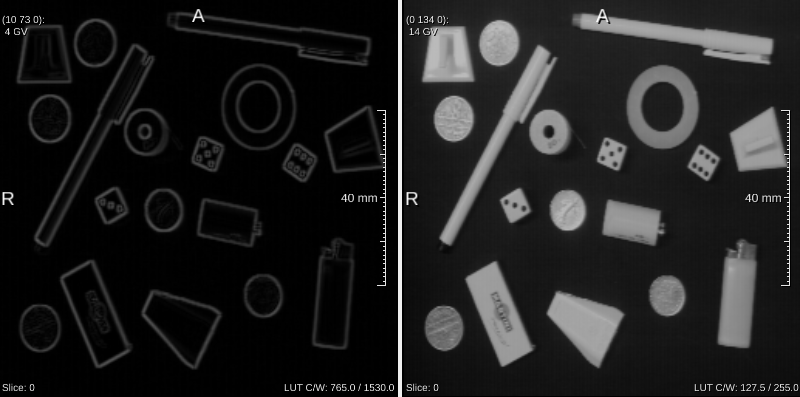
\includegraphics[width=0.7\textwidth]{1Filtros/1_prew_grad.png} % Include the image placeholder.png
\caption{Imagen original y su gradiente tipo Prewitt}
\label{fg:prewl_grad}
\end{center}
\end{figure}
\FloatBarrier

Para observar mejor las diferencias entre ambos operadores (uno lineal y el otro gaussiano)
realizamos la resta entre ambos y le hacemos una expansión del histograma para poder observar
mejor los resultados.

\begin{figure}[ht]
\centering
\begin{minipage}{.45\textwidth}
  \centering
    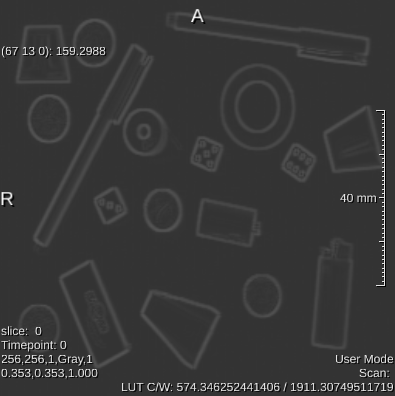
\includegraphics[width=0.7\textwidth]{1Filtros/1_prew_menos_sobel.png} % Include the image placeholder.png
\caption{Diferencia entre los gradientes de Prewitt y Sobel}
\label{fg:prewl_menos_sobel}
\end{minipage}%
\begin{minipage}{.45\textwidth}
  \centering
    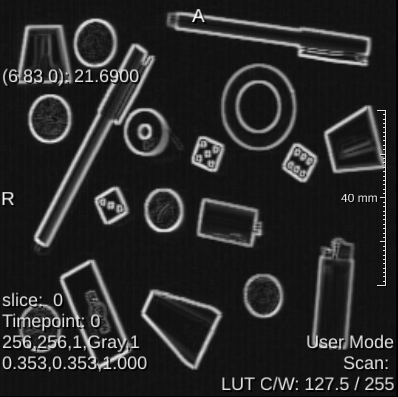
\includegraphics[width=0.7\textwidth]{1Filtros/1_prew_menos_sobel_scale.png} % Include the image placeholder.png
\caption{Diferencia entre los gradientes de Prewitt y Sobel luego de una expansión del histograma}
\label{fg:prewl_menos_sobel_scale}
\end{minipage}
\end{figure}
\FloatBarrier

Podemos observar claramente que hay una diferencia entre los valores calculados con el
operador de Sobel y los calculados con el operador de Prewitt. La diferencia recae en que el
operador de Sobel, siendo de forma Gaussiana de amplitud mayor a 1 (2, de hecho) va a
devolver valores calculados mayores que los calculados con el operador de Prewitt. Esta
diferencia se evidencia aún más en el siguiente ejercicio numérico:\\

Recordemos las máscaras de Sobel y de Prewitt.\\
Máscaras de Sobel
\[
g_x = 
\begin{bmatrix}
    -1 & -2 & -1\\
    0 & 0 & 0 \\
    1 & 2 & 1 
\end{bmatrix}
g_y = 
\begin{bmatrix}
    -1 & 0 & 1\\
    -2 & 0 & 2 \\
    -1 & 0 & 1 
\end{bmatrix}
\]
Máscaras de Prewitt:\\
\[
g_x = 
\begin{bmatrix}
    -1 & -1 & -1\\
    0 & 0 & 0 \\
    1 & 1 & 1 
\end{bmatrix}
g_y = 
\begin{bmatrix}
    -1 & 0 & 1\\
    -1 & 0 & 1 \\
    -1 & 0 & 1 
\end{bmatrix}
\]
Ahora calculemos $g_x$, $g_y$ y $g$ de Sobel y Preweitt para cada uno de los siguientes casos:\\
Frontera horizontal entre negro y blanco, 
\[ 
\begin{bmatrix}
    0 & 0 & 0\\
    0 & 0 & 0 \\
    255 & 255 & 255 
\end{bmatrix} 
\]

Para Sobel:
$
g_x = 4 * 255 = 1020
$
; 
$
g_y = - 255 + 255 = 0
$
 y 
$
g = |g_x| + |g_y| = 1020
$
\\
Para Prewitt:
$
g_x = 3 * 255 = 765
$
; 
$
g_y = - 255 + 255 = 0
$
 y 
$
g  = |g_x| + |g_y| = 765
$
\\

Frontera vertical entre negro y blanco, 
\[ 
\begin{bmatrix}
    0 & 0 & 255\\
    0 & 0 & 255 \\
    0 & 0 & 255 
\end{bmatrix} 
\]

Para Sobel:
$
g_x = -255 + 255 = 0
$
; 
$
g_y = 4*255 = 1020
$
 y 
$
g = |g_x| + |g_y| = 1020
$
\\
Para Prewitt:
$
g_x = - 255 + 255 = 0
$
; 
$
g_y = 3 * 255 = 765
$
 y 
$
g  = |g_x| + |g_y| = 765
$
\\

Frontera oblicua entre negro y blanco, 
\[ 
\begin{bmatrix}
    0   &  0  & 255 \\
    0   & 255 & 255 \\
    255 & 255 & 255 
\end{bmatrix} 
\]

Para Sobel:
$
g_x = -255 + 4 * 255 = 765
$
; 
$
g_y = -255 + 4 * 255 = 765
$
 y 
$
g = |g_x| + |g_y| = 1530
$
\\
Para Prewitt:
$
g_x = -255 + 3 * 255 = 510
$
; 
$
g_y = -255 + 3 * 255 = 510
$
 y 
$
g  = |g_x| + |g_y| = 1020
$
\\

Cuando la frontera se aleja de la frontera oblicua (máscara centrada en [0] 
\[ 
\begin{bmatrix}
    0   &  0   &  0  &  0  \\
    0   & [0]  &  0  & 255 \\
    0   &  0   & 255 & 255 \\
    0   &  255 & 255 & 255 
\end{bmatrix} 
\]

Para Sobel:
$
g_x =  255 
$
; 
$
g_y =  255
$
 y 
$
g = |g_x| + |g_y| = 510
$
\\
Para Prewitt:
$
g_x = 255
$
; 
$
g_y = 255
$
 y 
$
g  = |g_x| + |g_y| = 510
$
\\
\begin{par}
Podemos observar que al aplicar la máscara de Sobel en las fronteras obtenemos siempre
valores más elevados que al aplicar la máscara de Prewitt (debido a la gaussiana). 
También, la diferencia entre fronteras puramente verticales u horizaontales con frontera
oblicua es mayor (el doble) para la máscara de Sobel ($1530 - 1020 = 510$) que para la máscara de Prewitt ($1020 - 765 = 255$). Esto puede llegar a ser una ventaja ya que a mayor
diferencia aplicar una umbralización se facilita. 
Para el caso de estar alejados de la frontera podemos observar que ambas máscaras brindan los
mismos resultados. Podríamos entonces pensar que las fronteras se verán más marcadas pasando máscaras de Sobel que máscaras de Prewitt ya que da valores mayores en las fronteras. 
\end{par}
%----------------------------------------------------------------------------------------
%	Operador de Canny - Francisco
%----------------------------------------------------------------------------------------

\FloatBarrier
\section{Operador de Canny}

En esta sección se presentan los resultados obtenidos al aplicar el operador Canny sobre una imagen de prueba. En primer lugar, se aplica el operador Sobel sobre la imagen rondelle.png con la finalidad de observar los efectos de la detección de contornos bajo esta técnica. Los resultados son presentados en la figura \ref{fg:sobelOrig}.

\begin{figure}[ht]
\begin{center}
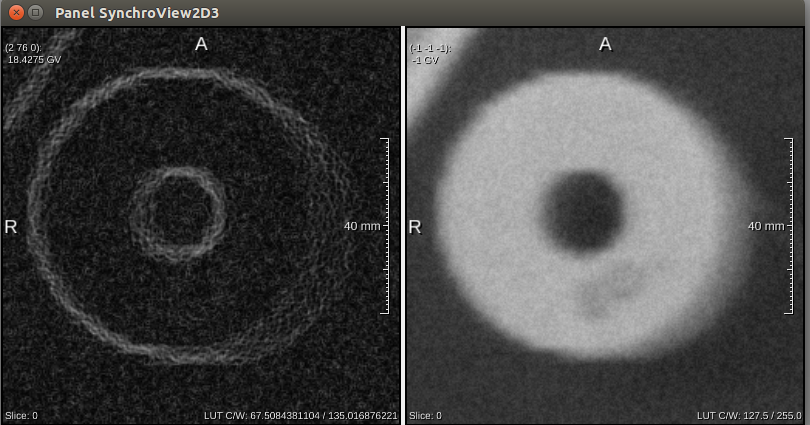
\includegraphics[width=0.9\textwidth]{2canny/2_sobel_orig} % Include the image placeholder.png
\caption{Imagen rondelle. Derecha: original. Izquierda: aplicación de operador Sobel}
\label{fg:sobelOrig}
\end{center}
\end{figure}
\FloatBarrier

En este caso, se observa que la imagen obtenida a partir de la magnitud del gradiente no es suficiente para la detección de contornos. Esto se debe, entre otros aspectos, al ruido característico de la imagen y a los contornos difusos de la estructura central. Es por este motivo que resulta necesaria la aplicación de un método que realice un proceso de filtrado previo con la finalidad de reducir el ruido. Adicionalmente, se requiere de un parámetro más estricto para la selección de los píxeles correspondientes al contorno. Es por este motivo que la aplicación del operador de Canny resulta más apropiada para este caso particular. En las figuras \ref{fg:canny1}, \ref{fg:canny2}, \ref{fg:canny3} y \ref{fg:canny4}. \\
En primer lugar, se observa en las figuras \ref{fg:canny1} y \ref{fg:canny2} la aplicación del operador con un valor de varianza de 1. A partir de este par de imágenes se pueden observar los efectos de aplicar diferentes niveles de umbral superior.

\begin{figure}[ht]
\centering
\begin{minipage}{.5\textwidth}
  \centering
  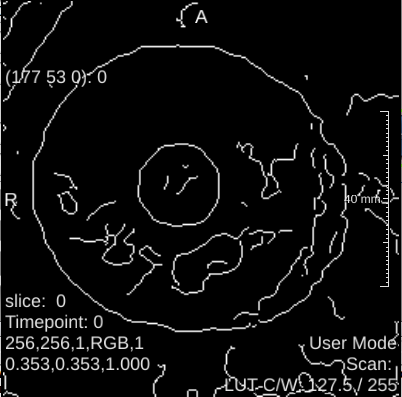
\includegraphics[width=0.8\textwidth]{2canny/2_canny_var_1_th_1_with_scale}
  \caption{var = 1, th = 1}
\label{fg:canny1}
\end{minipage}%
\begin{minipage}{.5\textwidth}
  \centering
  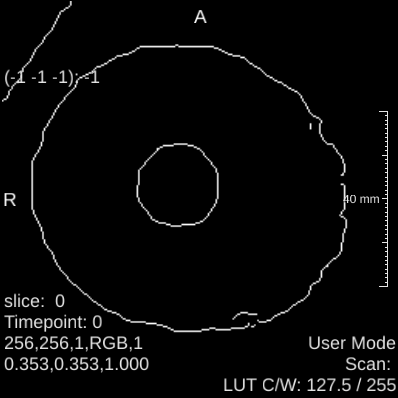
\includegraphics[width=0.8\textwidth]{2canny/2_canny_var_1_th_5_with_scale}
  \caption{var = 1, th = 5}
\label{fg:canny2}
\end{minipage}
\end{figure}
\FloatBarrier

En la imagen \ref{fg:canny1}, correspondiente a un nivel de th de 1, se observa la presencia de contornos falsos que no corresponden a la silueta de la imagen. Este efecto es producido debido a que el parámetro para la selección de bordes (umbral superior) no es lo suficientemente estricto para descartar estos contornos no deseados, que son producto de niveles de ruido al interior de la imagen. En la figura \ref{fg:canny2} se observan los efectos de incrementar el parámetro de umbral superior (th = 5). En este caso se observa que, al tener un parámetro de selección más estricto, se elimina la presencia de contornos falsos al interior de la estructura.

\begin{figure}[ht]
\centering
\begin{minipage}{.5\textwidth}
  \centering
  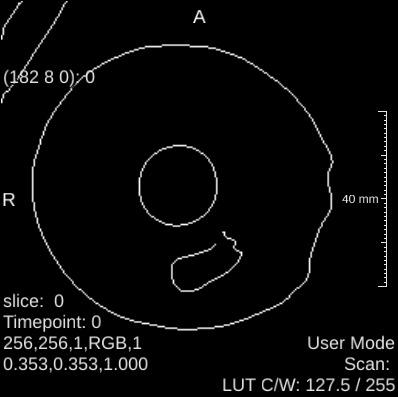
\includegraphics[width=0.8\textwidth]{2canny/2_canny_var_6_th_1_with_scale}
  \caption{var = 6, th = 1}
\label{fg:canny3}
\end{minipage}%
\begin{minipage}{.5\textwidth}
  \centering
  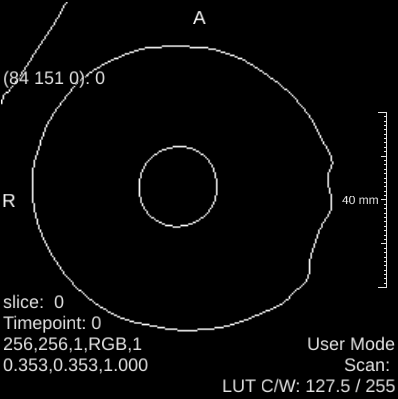
\includegraphics[width=0.8\textwidth]{2canny/2_canny_var_6_th_5_with_scale}
  \caption{var = 6, th = 5}
\label{fg:canny4}
\end{minipage}
\end{figure}
\FloatBarrier

Finalmente, en las figuras \ref{fg:canny3} y \ref{fg:canny4}, se observan los efectos de incrementar el valor de la varianza respecto a las figuras \ref{fg:canny1} y \ref{fg:canny2}. El efecto de incrementar el valor de la varianza a 6 corresponde a un mayor filtrado de la imagen. Esto se observa en los nuevos contornos de resultado, que se caracterizan por trazos más suavizados en relación a los obtenidos con una varianza de 1. Adicionalmente, este filtrado también contribuye a la reducción del ruido en la estructura, lo cual conlleva a la eliminación de trazos falsos al interior de la silueta. \\
Por último se observa que, en este caso, el mejor resultado es obtenido empleando los valores 6 y 5 para varianza y umbral superior respectivamente. Sin embargo, también es posible observar que el incremento de dichos parámetros no necesariamente conlleva a la obtención de mejores resultados. \\
El incremento excesivo de la varianza se traduce en un efecto de filtrado extremo que podría distorsionar la figura a analizar. Por otro lado el incremento extremo del umbral superior se traduce en un parámetro de selección excesivamente estricto, lo cual conllevaría al aumento de contornos no conexos en la definición de la silueta de la figura. Estos efectos son estudiados posteriormente en la sección del ejercicio de síntesis.

%----------------------------------------------------------------------------------------
%	Laplaciano - Sergio
%----------------------------------------------------------------------------------------

\section{Laplaciano}

\subsection{Ejercicio 1}

Recordemos la imagen inicial:

\begin{figure}[ht]
\begin{center}
    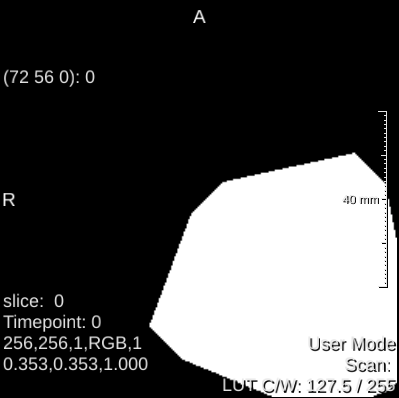
\includegraphics[width=0.4\textwidth]{3Laplaciano/3_spot_orig.png} % Include the image placeholder.png
    \caption{Imagen original}
\label{fg:spot_orig}
\end{center}
\end{figure}
\FloatBarrier

Aplicamos el LoG (Laplacian of a Gaussian). Al ser difícil la visualización, realizamos una expansión del histograma.

\begin{figure}[ht]
\centering
\begin{minipage}{.5\textwidth}
  \centering
    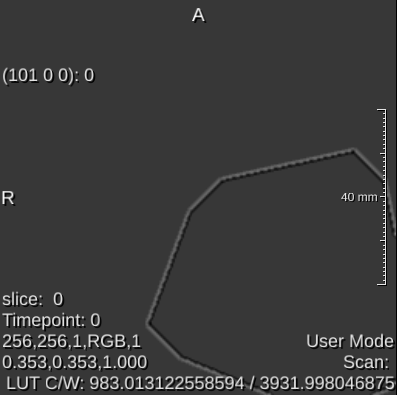
\includegraphics[width=0.7\textwidth]{3Laplaciano/3_ker_1_sigma_5.png} % Include the image placeholder.png
    \caption{LoG con Kernel Extent = 1 y Sigma = 0.5 aplicado en spot}
    \label{fg:spot_1_5}
\end{minipage}%
\begin{minipage}{.5\textwidth}
  \centering
  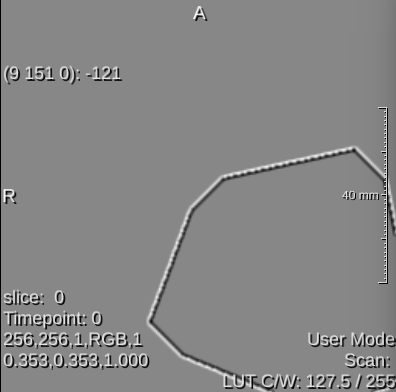
\includegraphics[width=0.7\textwidth]{3Laplaciano/3_ker_1_sigma_5_scale.png}
  \caption{LoG con Kernel Extent = 1 y Sigma = 0.5 aplicado en spot con histograma expandido}
\label{fg:spot_1_5_scale}
\end{minipage}
\end{figure}
\FloatBarrier

Podemos observar que en las regiones homogéneas el resultado es completamente negro (0) y en
los contornos obtenemos primero un valor muy positivo (blanco) y enseguida un valor muy
negativo (negro) pasando del negro al blanco. Esto se debe a que hubo un crecimiento muy
acentuado al pasar tan rápido del negro al blanco. Este crecimiento se traduce en un valor
positivo de la primera derivada (gradiente) justo en la frontera. Si observamos los cambios
de la primera derivada, primero es nula, luego crece muy rápidamente (un cambio positivo
fuerte) y luego disminuye muy rápidamente (un cambio negativo fuerte) hasta ser nula de
nuevo. Este cambio de la primera derivada se traduce en la segunda derivada, que se puede
observar en el LoG aplicado, primero es muy positivo (blanco) y luego muy negativo (negro) a
lo ancho de la frontera y nulo en el resto de la imagen.\\

\begin{figure}[ht]
\begin{center}
    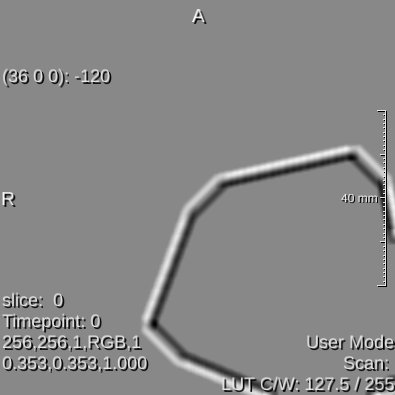
\includegraphics[width=0.4\textwidth]{3Laplaciano/3_ker_2_sigma_2.png} % Include the image placeholder.png
    \caption{LoG con Kernel Extent = 2 y Sigma = 2 aplicado en spot}
\end{center}
\end{figure}
\FloatBarrier

Al aumentar el sigma y el kernel extent podemos observar que el espesor de los contornos en la imagen aumentaron. Esto es debido a que la gaussiana usada en el LoG es ahora más ancha que antes.\\

Observemos ahora el resultado de aplicar el LoG sobre la imagen bruit.\\
\begin{figure}[ht]
\begin{center}
    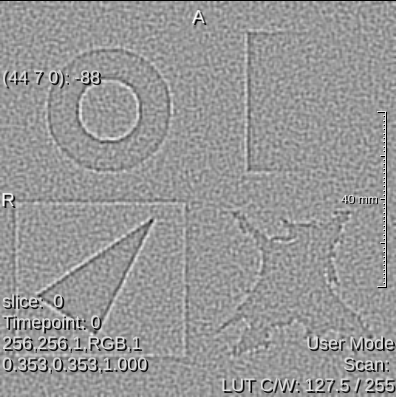
\includegraphics[width=0.4\textwidth]{3Laplaciano/3_bruit_ker_1_sigma_5.png} % Include the image placeholder.png
    \caption{LoG con Kernel Extent = 1 y Sigma = 0.5 aplicado en bruit}
\end{center}
\end{figure}
\FloatBarrier

Y lo comparamos con el resultado al aplicar el operador de Sobel (gradiente).\\
Observemos ahora el resultado de aplicar el LoG sobre la imagen bruit.\\
\begin{figure}[ht]
\begin{center}
    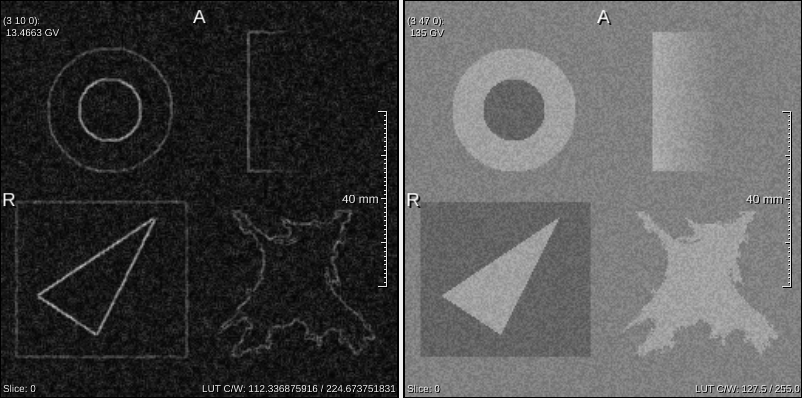
\includegraphics[width=0.6\textwidth]{3Laplaciano/3_bruit_sobel_grad.png} % Include the image placeholder.png
    \caption{Operador de Sobel aplicado en bruit con la imagen original}
\end{center}
\end{figure}
\FloatBarrier

Podemos observar que es más fácil detectar contornos en la imagen resultante del gradiente. 
Esto es debido a que la segunda derivada resalta el efecto del ruido en la imagen (y esta imagen tiene mucho), mucho más que el gradiente. En la imagen anterior, spot,  no se observo porque la imagen procesada no tiene ruido (es binaria).

\subsection{Ejercicio 2}

Aplicamos LoG a la imagen film. Obtenemos:

\begin{figure}[ht]
\centering
\begin{minipage}{.5\textwidth}
  \centering
    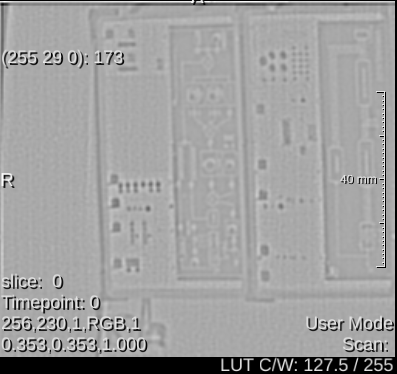
\includegraphics[width=0.7\textwidth]{3Laplaciano/3_film_LoG.png} % Include the image placeholder.png
    \caption{LoG con Kernel Extent = 1 y Sigma = 0.5 aplicado en film}
\end{minipage}%
\begin{minipage}{.5\textwidth}
  \centering
  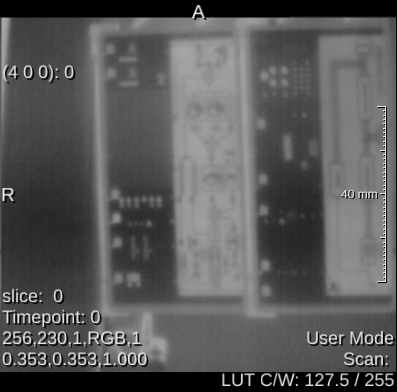
\includegraphics[width=0.7\textwidth]{3Laplaciano/3_film_orig.png}
  \caption{Imagen original}
\end{minipage}
\end{figure}
\FloatBarrier

Finalmente visualizamos la suma de 60\% de la imagen original con el resultado del LoG. 

\begin{figure}[ht]
\begin{center}
    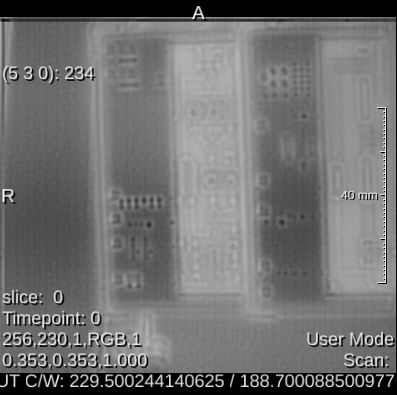
\includegraphics[width=0.5\textwidth]{3Laplaciano/3_film_6_orig_LoG.png} % Include the image placeholder.png
    \caption{Resultado luego de la expansión del historgrama}
\end{center}
\end{figure}
\FloatBarrier

Podemos observar que el resultado es bastante bueno y no parece tener tanto ruido como se esperaría ya que el LoG acentua el ruido en la imagen.\\

Ahora observemos el resultado luego de efectuar la misma operación salvo que la imagen original está ecualizada y la imagen combinada también.\\

Observemos ahora el resultado de aplicar el LoG sobre la imagen bruit. Realizamos una expansión del histograma para facilitar la visualización.\\
\begin{figure}[ht]
\begin{center}
    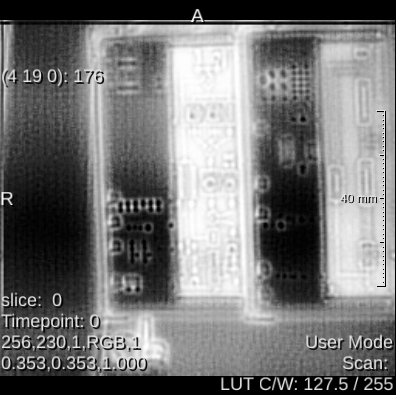
\includegraphics[width=0.5\textwidth]{3Laplaciano/3_film_ecual_both_scale.png} % Include the image placeholder.png
    \caption{Resultado, con las ecualizaciones}
\end{center}
\end{figure}
\FloatBarrier

Podemos observar que la ecualización mejora el contraste y los contornos se observan mejor en este resultado. \\
Podemos entonces concluir que combinaciones (suma del LoG con imagen original, ecualización) de operaciones pueden resultar con mejores resultados que únicamente calcular el Laplaciano ya que este último tiene sus riesgos (esencialmente, su ampliación del ruido).


%----------------------------------------------------------------------------------------
%	Ejercicio de Síntesis - Francisco
%----------------------------------------------------------------------------------------

\FloatBarrier
\section{Ejercicio de síntesis}

Con la finalidad de realizar el ejercicio de síntesis propuesto (enmarcar la figura en un contorno claro), se decidió emplear el Operador de Canny como método principal para obtener el contorno. Posteriormente, por medio de operaciones aritméticas, se realizó la síntesis de la imagen deseada. Los pasos realizados en este proceso son presentados a continuación. En primer lugar, se aplica el filtro de detección de contornos de Canny.\\ 
Los parámetros del filtro fueron calculados empíricamente con la finalidad de obtener el resultado deseado. En particular, se realizó un análisis sobre el comportamiento de la imagen resultado en términos del valor de varianza del filtro gaussiano y de los valores de threshold superior e inferior con la finalidad de determinar los píxeles pertenecientes al borde. \\
En este caso, se determinó un valor de 0.2 tanto para la varianza en x como para la varianza en y, los valores asociados a los umbrales superior e inferior corresponden a 2 y 0 respectivamente. La imagen resultante al aplicar este filtro, luego de ser procesada bajo una calibración de los niveles de gris (0-1 a 0-255), es presentada en la figura \ref{fg:resCanny}. \\
En particular, se realiza la evaluación del comportamiento del filtro bajo valores superiores e inferiores en todos los parámetros con el propósito de justificar la decisión de selección. los resultados obtenidos son presentados a continuación.

\begin{figure}[ht]
\begin{center}
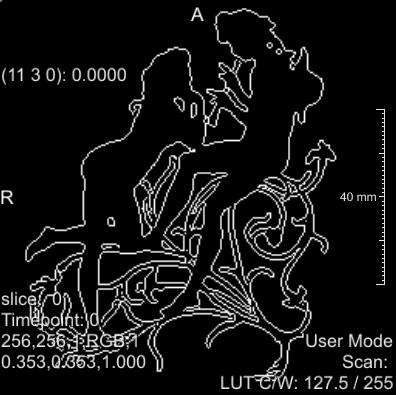
\includegraphics[width=0.5\textwidth]{4sintesis/canny.png} % Include the image placeholder.png
\caption{Resultado de aplicación: filtro de detección de contornos de Canny (varx = 0.2, vary = 0.2, th = 2, tl = 0)}
\label{fg:resCanny}
\end{center}
\end{figure}
\FloatBarrier

En las figuras \ref{fg:cannyvar01} y \ref{fg:cannyvar05} se hacen evidentes los efectos de disminuir e incrementar la varianza del filtro gaussiano respectivamente. En la figura \ref{fg:cannyvar01}, se observa que al reducir la varianza del filtro no se logra contrarrestar el ruido de la imagen original, por lo tanto se generan contornos internos que no corresponden a la forma de la silueta. \\
Por otro lado, en la figura \ref{fg:cannyvar05}, se observa que al aumentar la varianza se consigue un efecto exagerado del filtro. Es por esta razón que se observan ciertas distorsiones en la forma del contorno de la figura respecto a la imagen original. A partir de estas observaciones, se determinó que el valor más adecuado para la varianza del filtro corresponde a 0.2 en ambas coordenadas.

\begin{figure}[ht]
\centering
\begin{minipage}{.5\textwidth}
  \centering
  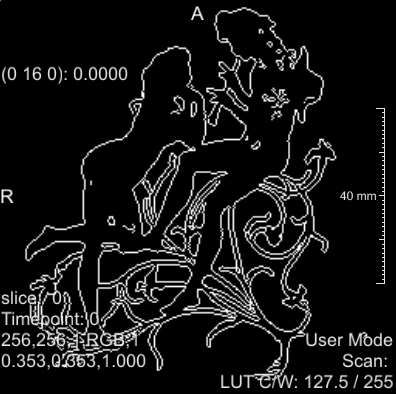
\includegraphics[width=0.8\textwidth]{4sintesis/cannyvar01.png}
  \caption{varx = 0.1, vary = 0.1, th = 2, tl = 0}
\label{fg:cannyvar01}
\end{minipage}%
\begin{minipage}{.5\textwidth}
  \centering
  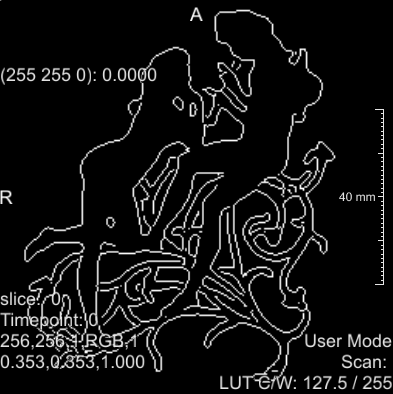
\includegraphics[width=0.8\textwidth]{4sintesis/cannyvar05.png}
  \caption{varx = 0.5, vary = 0.5, th = 2, tl = 0}
\label{fg:cannyvar05}
\end{minipage}
\end{figure}
\FloatBarrier

Posteriormente, se realiza el estudio de la variación de los parámetros umbral superior y umbral inferior. En primer lugar, se analizan los efectos de aumentar y disminuir el parámetro de umbral superior. Los resultados obtenidos son presentados en las figuras \ref{fg:cannyvar80} y \ref{fg:cannyvar10} respectivamente.

\begin{figure}[ht]
\centering
\begin{minipage}{.5\textwidth}
  \centering
  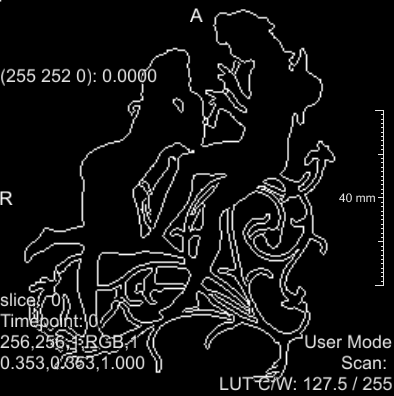
\includegraphics[width=0.8\textwidth]{4sintesis/cannyu8l0.png}
  \caption{varx = 0.2, vary = 0.2, th = 8, tl = 0}
\label{fg:cannyvar80}
\end{minipage}%
\begin{minipage}{.5\textwidth}
  \centering
  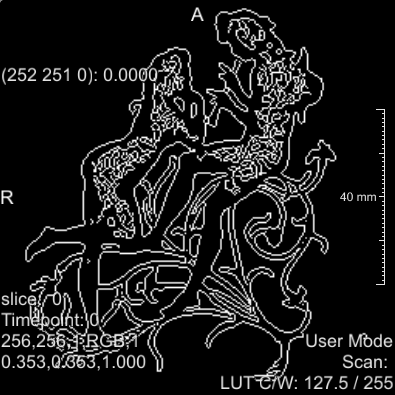
\includegraphics[width=0.8\textwidth]{4sintesis/cannyu1l0.png}
  \caption{varx = 0.2, vary = 0.2, th = 1, tl = 0}
\label{fg:cannyvar10}
\end{minipage}
\end{figure}
\FloatBarrier

En la figura \ref{fg:cannyvar80}, se observan los efectos de incrementar el valor de umbral superior. En este caso, se observa que al establecer un parámetro más exigente para la selección de contornos se pierden algunos detalles de la figura, particularmente detalles internos. Por otro lado en la figura \ref{fg:cannyvar10} se observa que, al disminuir el parámetro, se genera al interior de la imagen una serie de contornos que no corresponden a la silueta deseada. Esto se debe a que, al tener un criterio menos exigente, clasifican como bordes algunos píxeles asociados a niveles de ruido que no fueron satisfactoriamente filtrados. \\
Finalmente, se presentan los efectos de aumentar el criterio de umbral inferior en la figura \ref{fg:cannyvar10}. En este caso, la diferencia entre los resultados obtenidos respecto a la figura \ref{fg:resCanny} no resulta evidente. Sin embargo, luego de una inspección detallada de la imagen, se observa que al aumentar este parámetro se incrementa la cantidad de bordes no conectados. Esto también conlleva a una pérdida no deseada de detalles en la silueta.

\begin{figure}[ht]
\begin{center}
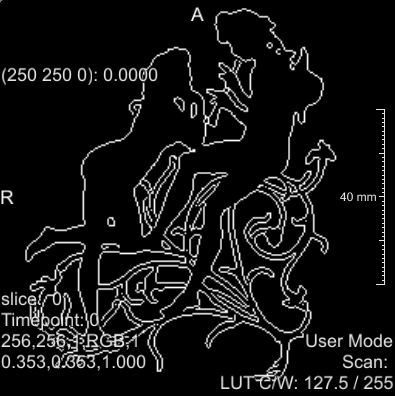
\includegraphics[width=0.4\textwidth]{4sintesis/cannyu2l2.png} % Include the image placeholder.png
\caption{Resultado de aplicación: filtro de detección de contornos de Canny (varx = 0.2, vary = 0.2, th = 2, tl = 2)}
\label{fg:cannyvar22}
\end{center}
\end{figure}
\FloatBarrier

Finalmente, se realiza una operación de OR entre la imagen resultante presentada en la figura \ref{fg:resCanny} y la imagen original para obtener el efecto deseado. Los resultados finales son presentados en la figura \ref{fg:finSintesis}.

\begin{figure}[ht]
\begin{center}
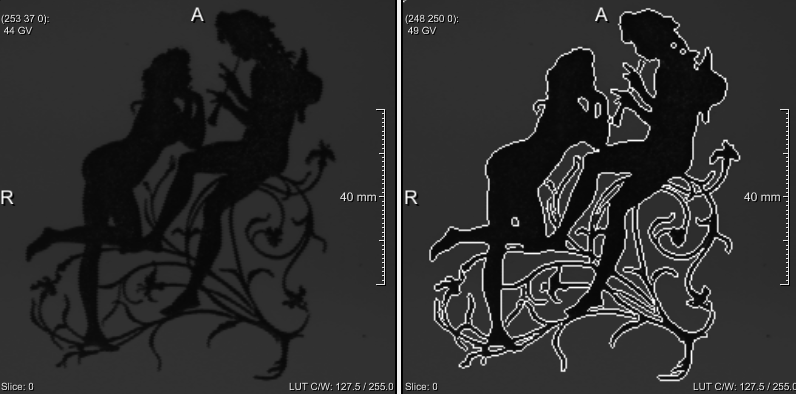
\includegraphics[width=1.0\textwidth]{4sintesis/cannyfinal.png} % Include the image placeholder.png
\caption{Resultado final (Operación OR entre imagen original e imagen presentada en figura \ref{fg:resCanny}}
\label{fg:finSintesis}
\end{center}
\end{figure}
\FloatBarrier

%----------------------------------------------------------------------------------------
%	BIBLIOGRAPHY
%----------------------------------------------------------------------------------------
\nocite{*}
\FloatBarrier

\bibliographystyle{abbrv}

\bibliography{sample}

%----------------------------------------------------------------------------------------

\end{document}